\documentclass[../defence.tex]{subfiles}
\begin{document}

  \begin{frame}{Graphitstrukturen}
    \begin{columns}[onlytextwidth, T]
      \column{\dimexpr\linewidth / 10 * 7}
        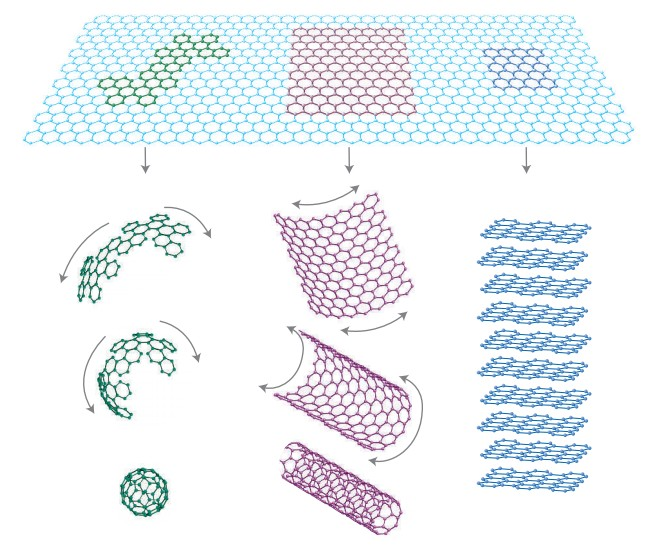
\includegraphics[width=\linewidth]{images/graphit.png}

      \column{\dimexpr\linewidth / 10 * 7}
        \cite{geim2007}
    \end{columns}
    \note{
      \begin{itemize}
        \item nanotubes (1D), Fullerene (0D), Graphit (3D)
        \item Monolagen bisher kaum herstellbar $\rightarrow$ wie viele Lagen können als 2D Struktur betrachtet werden?
        \item Elektronische Struktur ändert sich rapide bei Erreichen von 10 Schichten  \\
              Bis zu 2 Schichten $\rightarrow$ 1 Ladungsträgertyp, 1 Lochtyp (simples elektronisches Spektrum);\\
              3+ Schichten $\rightarrow$ mehrere Ladungsträger- und Lochtypen (kompliziertes elektronisches Spektrum);
        \item $\Rightarrow$ 1, 2, 3+<10 Lagenstrukturen in 3 2D Kristalle unterscheidbar
      \end{itemize}}
  \end{frame}

\end{document}
